\section{LHC New Physics Dataset}
{{\footnotesize
\begin{description}[labelwidth=5em, labelsep=1em, leftmargin=*, align=left, itemsep=0.3em, parsep=0em]
  \item[date:] 2021-07-05
  \item[version:] TODO
  \item[last\_updated:] 2021-07
  \item[expired:] unknown
  \item[valid:] yes
  \item[valid\_date:] TODO
  \item[url:] \href{https://arxiv.org/pdf/2107.02157}{https://arxiv.org/pdf/2107.02157}
  \item[doi:] TODO
  \item[domain:] Particle Physics; Real-time Triggering
  \item[focus:] Real-time LHC event filtering for anomaly detection using proton collision data
  \item[keywords:]
    - anomaly detection
    - proton collision
    - real-time inference
    - event filtering
    - unsupervised ML
  \item[summary:] A dataset of proton-proton collision events emulating a 40 MHz real-time data stream from LHC detectors, pre-filtered on electron or muon presence. Designed for unsupervised new-physics detection algorithms under latency/bandwidth constraints.

  \item[licensing:] TODO
  \item[task\_types:]
    - Anomaly detection
    - Event classification
  \item[ai\_capability\_measured:]
    - Unsupervised signal detection under latency and bandwidth constraints
  \item[metrics:]
    - ROC-AUC
    - Detection efficiency
  \item[models:]
    - Autoencoder
    - Variational autoencoder
    - Isolation forest
  \item[ml\_motif:]
    - Multiple
  \item[type:] Framework
  \item[ml\_task:]
    - NA
  \item[solutions:] TODO
  \item[notes:] Includes electron/muon-filtered background and black-box signal benchmarks; 1M events per black box.

  \item[contact.name:] Ema Puljak (ema.puljak@cern.ch)
  \item[contact.email:] unknown
  \item[datasets.links.name:] Zenodo stores, background + 3 black-box signal sets. 1M events each
  \item[results.links.name:] ChatGPT LLM
  \item[fair.reproducible:] Yes
  \item[fair.benchmark\_ready:] Yes
  \item[ratings.software.rating:] 0
  \item[ratings.software.reason:] Not analysed. 

  \item[ratings.specification.rating:] 7.0
  \item[ratings.specification.reason:] The problem (anomaly detection for new physics at LHC) is clearly described with goals and background, but lacks a formal task specification or constraints.

  \item[ratings.dataset.rating:] 8.0
  \item[ratings.dataset.reason:] Large-scale, public dataset derived from LHC simulations; well-documented and available via Zenodo.

  \item[ratings.metrics.rating:] 7.0
  \item[ratings.metrics.reason:] Provides AUROC, accuracy, and anomaly detection metrics but lacks standardized evaluation script.

  \item[ratings.reference\_solution.rating:] 5.0
  \item[ratings.reference\_solution.reason:] Baseline models (autoencoders, GANs) are described in associated papers, but implementations vary across papers.

  \item[ratings.documentation.rating:] 6.0
  \item[ratings.documentation.reason:] Publicly available papers and datasets with descriptions, but no unified README or training setup.

  \item[id:] lhc\_new\_physics\_dataset
  \item[Citations:] \cite{https://doi.org/10.5281/zenodo.5046389}
  \item[Ratings:]
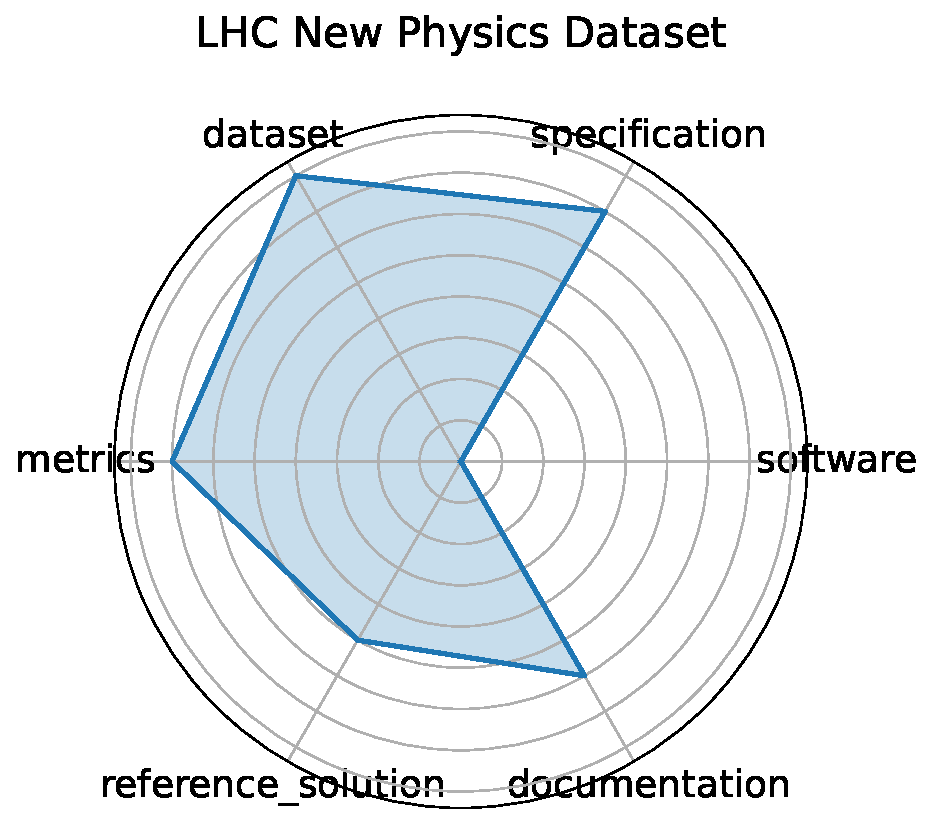
\includegraphics[width=0.2\textwidth]{lhc_new_physics_dataset_radar.pdf}
\end{description}
}}
\clearpage